\section{Dashboard Using R}

\subsection*{Why Dashboards?}
A dashboard acts like a control panel for your data, showing the most important trends and statistics at a glance. In climate data analysis, dashboards can help track real-time changes in temperature, humidity, or rainfall and communicate findings visually.

\subsection*{Creating a Climate Dashboard with R}
Creating a visual and interactive dashboard is an excellent way to explore and communicate insights from climate data. In this section, we will walk through how to create a climate dashboard using \texttt{flexdashboard}, \texttt{ggplot2}, and \texttt{lubridate} packages in R.

\subsubsection*{1. Installing Required Packages}
Before proceeding, ensure the necessary packages are installed. Run the following commands in your R console:
\begin{verbatim}
install.packages("ggplot2") 
install.packages("flexdashboard") 
install.packages("lubridate")
\end{verbatim}

These packages serve the following purposes:
\begin{itemize}
    \item \textbf{ggplot2} — for creating advanced visualizations.
    \item \textbf{flexdashboard} — for building dashboards using R Markdown.
    \item \textbf{lubridate} — for handling and manipulating date-time data.
\end{itemize}

\subsubsection*{2. Loading Your Climate Dataset}
Prepare your dataset in CSV format. Suppose the file is named \texttt{dataframe.csv}. Load it into R using:

\begin{verbatim}
climate_data <- read.csv("dataframe.csv")
\end{verbatim}

This command reads the CSV file and stores it in the object \texttt{climate\_data}, which we will use for visualization.

\subsubsection*{3. Creating the FlexDashboard File}
\begin{enumerate}
  \item Open Visual Studio Code (VSCode) or RStudio. 
  \item Create a new file named \texttt{dashboard.Rmd}.

  \item At the top of the file, include the following YAML header:

\begin{verbatim}
---
title: "My Climate Data Dashboard"
output: 
  flexdashboard::flex_dashboard
runtime: shiny
---
\end{verbatim}
\end{enumerate}
This YAML header defines the document title, output format, and specifies that the dashboard will have interactive capabilities using Shiny.

\subsubsection*{4. Adding Plots to the Dashboard}

Use R code chunks within the R Markdown file to include visualizations. Here’s how you can organize two plots in the first row of your dashboard:

\textbf{Row 1: Temperature Histogram (Left) and Precipitation Bar Plot (Right)}

\begin{verbatim}
```{r}

# Left Column: Temperature Histogram

ggplot(climate_data, aes(x =Temp_2m)) +
geom_histogram(binwidth =1, fill ="skyblue",color ="black",alpha = 0.7)+
labs(
  title ="Temperature Histogram", 
  x = "Temperature (°C)", 
  y ="Density")+
  theme_minimal()

# Right Column: Precipitation Histogram

ggplot(climate_data, aes(x = Precip)) +
geom_histogram(binwidth =1,fill ="skyblue",color ="black",alpha = 0.7)+
labs(
  title = "Precipitation Histogram",
  x ="Precipitation",
  y = "Density")+
  theme_minimal()

\end{verbatim}

\subsubsection*{5. Rendering the Dashboard}
\begin{enumerate}
\item Once you have completed your \texttt{.Rmd} file with all necessary code chunks:
\item Save the file.
\item Render it in the R terminal by typing:
\begin{verbatim}
rmarkdown::render('d:/R project/dashboard.Rmd')
\end{verbatim}
\end{enumerate}

This will generate an HTML output of the dashboard.

\subsubsection*{6. Viewing the Dashboard}
Navigate to the location where the HTML file is saved. Open it using any web browser. You should see an interactive dashboard displaying the plots you’ve created.

% Figure here--------------------------
\begin{figure}[h]
\centering
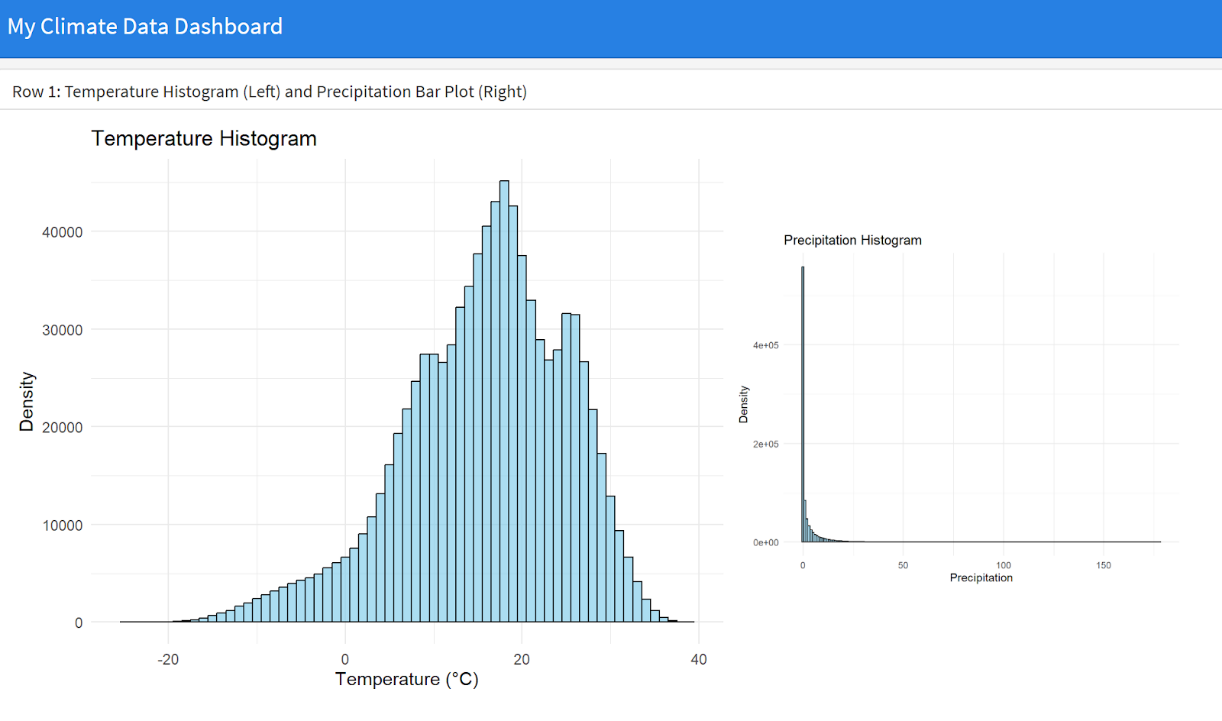
\includegraphics[width=0.8\textwidth]{figures/dashboard.png}
\caption{Figure 7.2: Dashboard using R}
\end{figure}

\subsection*{Summary Checklist for Learners}
\begin{itemize}
\item Installed required packages (\texttt{ggplot2}, \texttt{flexdashboard}, \texttt{lubridate})
\item Loaded and verified climate data
\item Created an R Markdown file with the correct YAML header
\item Added at least two informative visualizations
\item Rendered and opened the dashboard
\end{itemize}

\subsection*{Next Steps}
Try adding more components such as:
\begin{itemize}
\item Time series plots for temperature trends.
\item Interactive filters using Shiny widgets.
\item Value boxes showing summary statistics.
\end{itemize}
